\hypertarget{SoundSample_8cpp}{
\section{Sound\-Sample.cpp File Reference}
\label{SoundSample_8cpp}\index{SoundSample.cpp@{SoundSample.cpp}}
}
{\tt \#include \char`\"{}Sound\-Sample.h\char`\"{}}\par


Include dependency graph for Sound\-Sample.cpp:\begin{figure}[H]
\begin{center}
\leavevmode
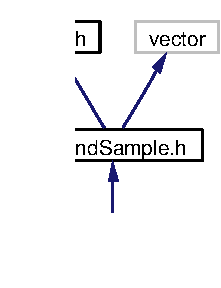
\includegraphics[width=70pt]{SoundSample_8cpp__incl}
\end{center}
\end{figure}
\subsection*{Defines}
\begin{CompactItemize}
\item 
\#define \hyperlink{SoundSample_8cpp_a0}{MIN\_\-CLIP\_\-WARNING}\ 10
\end{CompactItemize}


\subsection{Define Documentation}
\hypertarget{SoundSample_8cpp_a0}{
\index{SoundSample.cpp@{Sound\-Sample.cpp}!MIN_CLIP_WARNING@{MIN\_\-CLIP\_\-WARNING}}
\index{MIN_CLIP_WARNING@{MIN\_\-CLIP\_\-WARNING}!SoundSample.cpp@{Sound\-Sample.cpp}}
\subsubsection[MIN\_\-CLIP\_\-WARNING]{\setlength{\rightskip}{0pt plus 5cm}\#define MIN\_\-CLIP\_\-WARNING\ 10}}
\label{SoundSample_8cpp_a0}


Because m\_\-time\_\-type is a float, there can be a slight round-off error that causes different calculations to produce different numbers of samples for a given Track/Sound\-Sample. We would like to warn the user if he tries to composite two sections of vastly different lengths, but we need to have some acceptable error to account for round-off errors inherent in the program and not caused by users 

Definition at line 43 of file Sound\-Sample.cpp.

Referenced by Sound\-Sample::composite().